
\documentclass[11pt, aspectratio=169]{beamer}
%\documentclass[draft, 11pt, aspectratio=169]{beamer}

% --- Preamble Settings ---
\usepackage[english]{babel}
\usepackage{textcomp} % Required for some characters inside verbatim/code
\usepackage{amsmath} % For math environments
\usepackage{booktabs} % For nice tables
\usepackage{subfig}
\usepackage{fontawesome5} % for icons
\usepackage{hyperref}     % clickable links
% Load TikZ
\usepackage{tikz}
%\usetikzlibrary{arrows.meta,positioning} % for Stealth arrow tips & node positioning
%\usepackage{tikz}
\usetikzlibrary{positioning,shapes,arrows.meta,fit,backgrounds}
\setbeamertemplate{navigation symbols}{}

\usepackage{pgfpages}
\usepackage{pgfpages}
\ifdefined\shownotes
  \setbeameroption{show notes on second screen=right}
\else
  \setbeameroption{hide notes}
\fi

% --- Theme and Appearance ---
% The 'Boadilla' theme is clean and professional.
%\usetheme{Berlin} 
\usetheme{Singapore} 
%\usetheme{Barcelona}
\setbeamertemplate{footline}{} 
\setbeamertemplate{navigation symbols}{}
\AtBeginSection{
  \begin{frame}[plain]
    \centering
    \vspace{2cm}
    {\Huge \insertsection}
  \end{frame}
}

% Add logos to the title page only (bottom left & bottom right)
\addtobeamertemplate{title page}{}{% appended at end of the title page
  \begin{tikzpicture}[remember picture,overlay]
    % left logo
    \node[anchor=south west] at
      ([xshift=0.6cm,yshift=0.6cm]current page.south west)
      {
\includegraphics[height=1.0cm]{cogs_logo}}; % e.g., cogs_logo.png/pdf
    % right logo
    \node[anchor=south east] at
      ([xshift=-0.6cm,yshift=0.6cm]current page.south east)
      {
\includegraphics[height=1.0cm]{sdsu_logo}}; % e.g., sdsu_logo.png/pdf
  \end{tikzpicture}
}




%\usecolortheme{beaver} % Light background, good contrast
\title{SDSS26}
\subtitle{Designing a Durable Open Source Ecosystem for Spatial Data Science}
\date{March 15-16, 2026}


% --- A small helper macro for a module tile (image + title + link)
\newcommand{\modtile}[3]{% #1=title, #2=image file, #3=url
  \href{#3}{%
    \begin{minipage}[t]{0.235\linewidth}
      \centering
      \includegraphics[width=\linewidth,height=0.70\linewidth,keepaspectratio]{#2}\\[2pt]
      \bfseries #1
    \end{minipage}%
  }%
}
% --- Custom Commands (Optional) ---
%
%\setbeamertemplate{footline}{%
%  \leavevmode%
%  \hbox{%
%    \begin{beamercolorbox}[wd=.3333\paperwidth,ht=2.25ex,dp=1ex,center]{author in head/foot}%
%      \usebeamerfont{author in head/foot}\insertauthor
%    \end{beamercolorbox}%
%    \begin{beamercolorbox}[wd=.3333\paperwidth,ht=2.25ex,dp=1ex,center]{title in head/foot}%
%      \usebeamerfont{title in head/foot}\insertshorttitle{}
%    \end{beamercolorbox}%
%    \begin{beamercolorbox}[wd=.3333\paperwidth,ht=2.25ex,dp=1ex,right]{date in head/foot}%
%      \insertframenumber{} / \inserttotalframenumber\hspace*{2ex}
%    \end{beamercolorbox}}%
%  \vskip0pt%
%}

% Add one or more directories (must end with /)
\graphicspath{{figures/}{images/}{graphics/}}

% --- Document Start ---
\begin{document}

% ----------------------------------------------------
% Slide 1: Title Page
% ----------------------------------------------------
\begin{frame}
    \titlepage
\end{frame}

\begin{frame}
  \tableofcontents
\end{frame}

\section{Why?} % 2 min
\note{10 minutes

  motivation, pysal origin story
  current challenges
  current opportunities
  project goals and framework
}

\begin{frame}{Spatial Data Science: Definition}
    
    \centering
    \Large
    Spatial Data Science = Data Science + Location + Geography
    \par\vspace{1em}
    \small
    We analyze patterns, predict outcomes, and model relationships while explicitly accounting for \textbf{spatial structure}.
    
    %\pause\vspace{1.5em}

    %\begin{table}
    %    \centering
    %    \begin{tabular}{lll}
    %        \toprule
    %        \textbf{Spatial Concept} & \textbf{Description} & \textbf{PySAL Tool} \\
    %        \midrule
    %        \textbf{Spatial Dependence} & Value at one location relates to nearby values (clustering). & \texttt{esda.moran} \\
    %        \pause
    %        \textbf{Spatial Heterogeneity} & Relationships change across space. & \texttt{giddy.markov} \\
    %        \bottomrule
    %    \end{tabular}
    %    \caption{Core Concepts and PySAL Modules}
    %\end{table}

\end{frame}



\begin{frame}{PySAL}
  
  \centering
  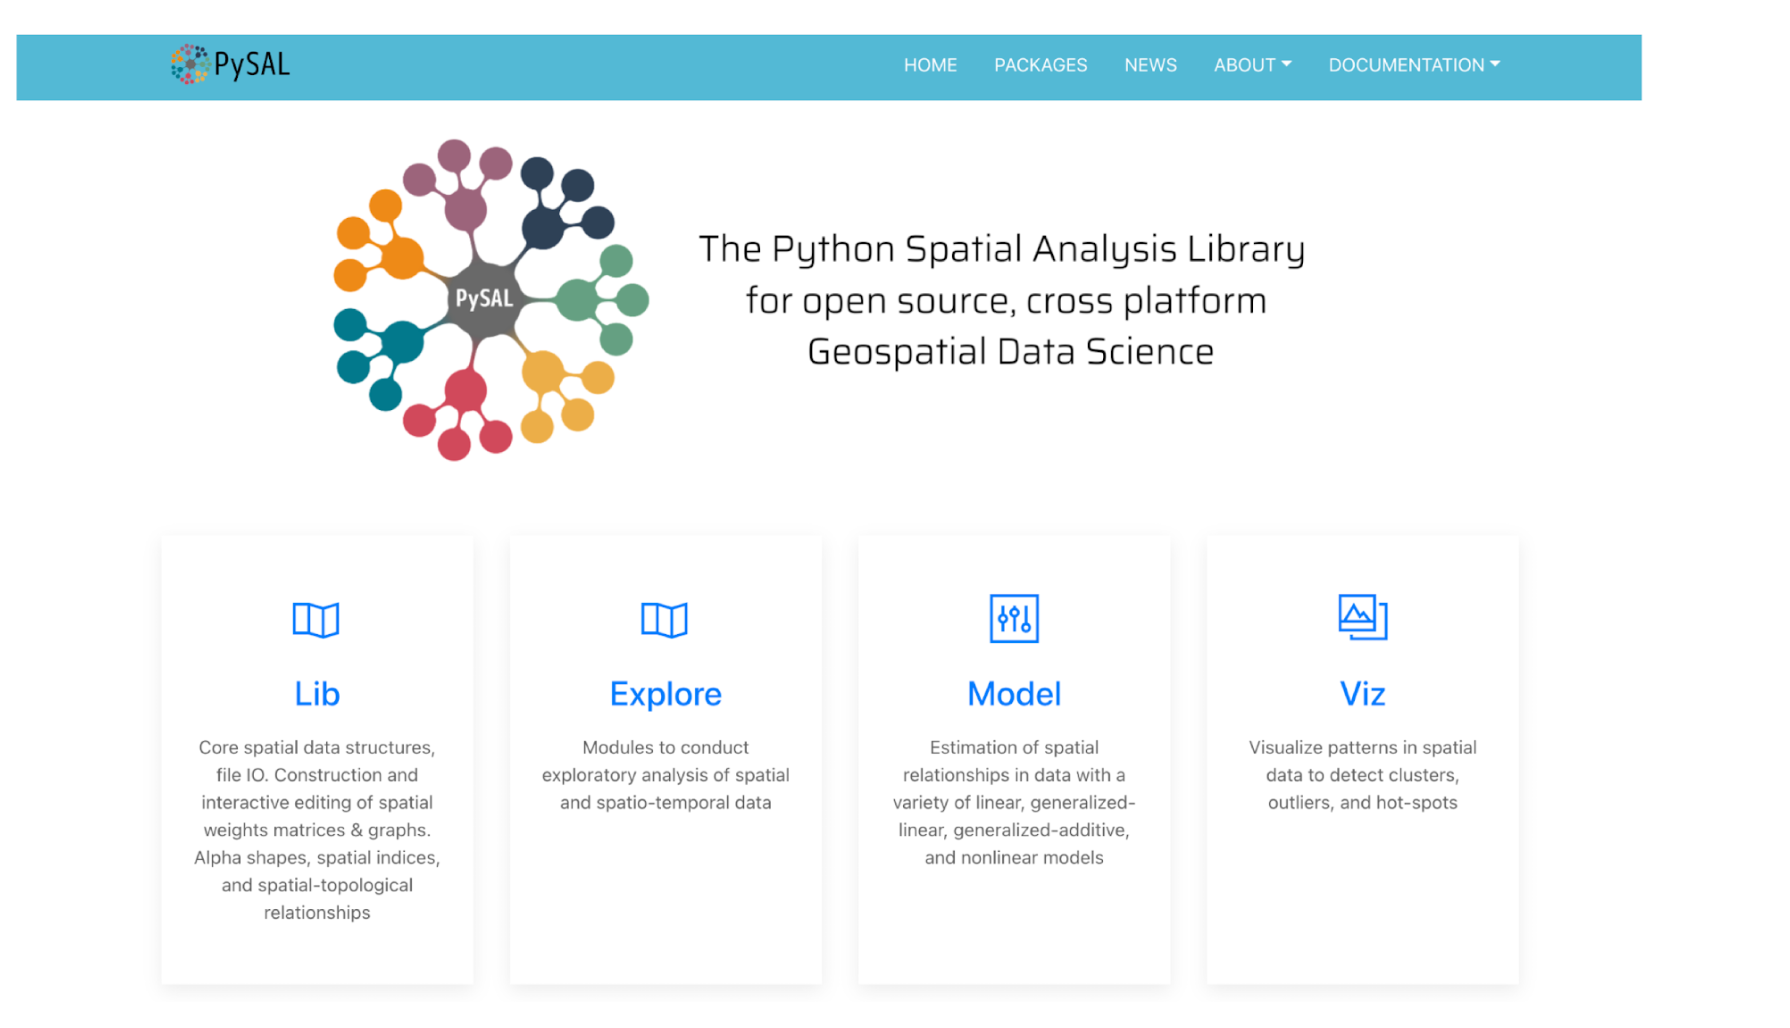
\includegraphics[width=0.8\linewidth]{figures/pysallayers.png} 
  
\end{frame}

\begin{frame}{History}
  \centering
  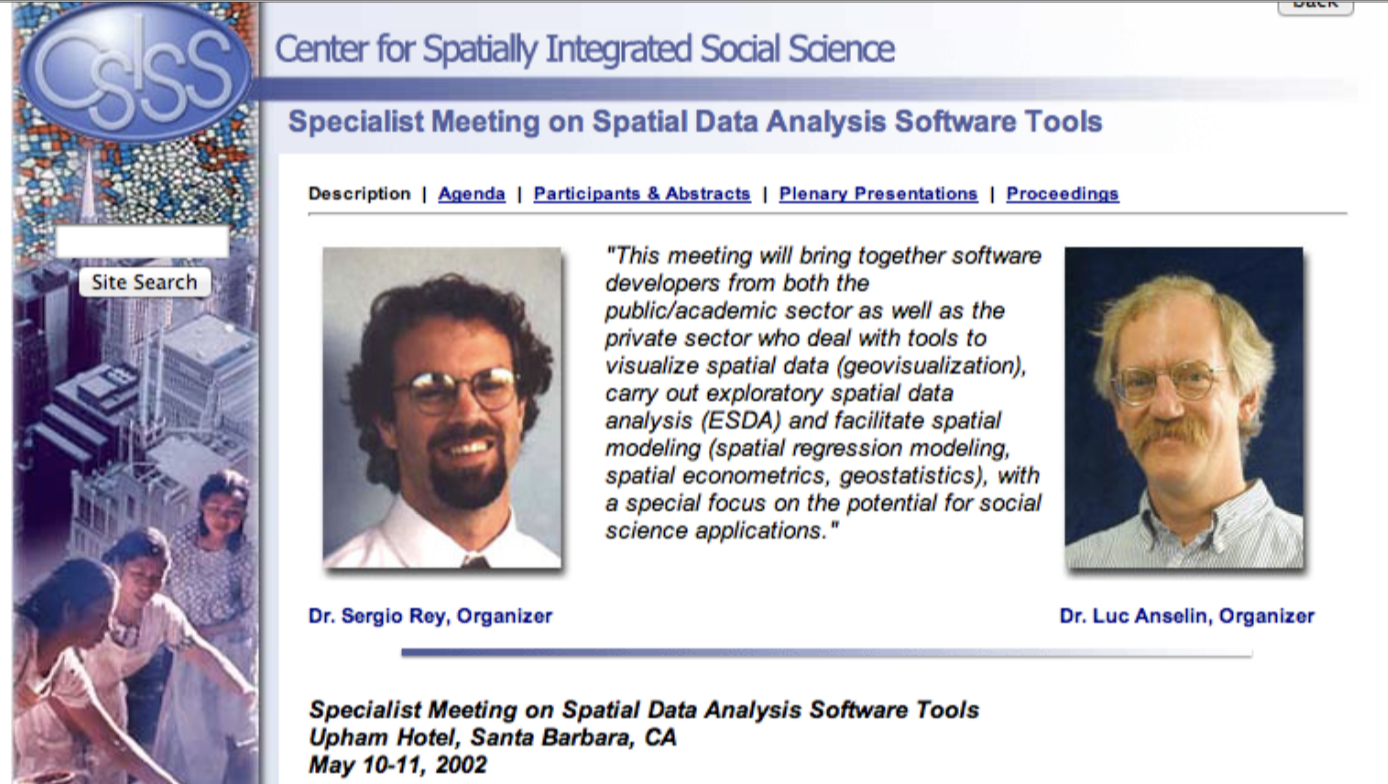
\includegraphics[width=0.8\linewidth]{figures/ancienthistory.png} 
\end{frame}


\begin{frame}\frametitle{PySAL Objectives (circa 2002)}
  \begin{block}{Leverage Existing Tools Development}
    \begin{itemize}
      \item GeoDa/PySpace
      \item STARS
    \end{itemize}
  \end{block}
  \begin{block}{Develop Core Library}
    \begin{itemize}
      \item spatial data \emph{analytical} functions
      \item enhanced specialization, modularity
      \item fill void in geospatial Python libraries
    \end{itemize}
  \end{block}
  \begin{block}{Flexible Delivery Mechanisms}
    \begin{itemize}
      \item interactive shell
      \item GUI/Toolkits (ArcGIS, QGIS)
      \item webservices
    \end{itemize}
  \end{block}
\end{frame}

% \begin{frame}\frametitle{Precursor}
%   \begin{center}
%     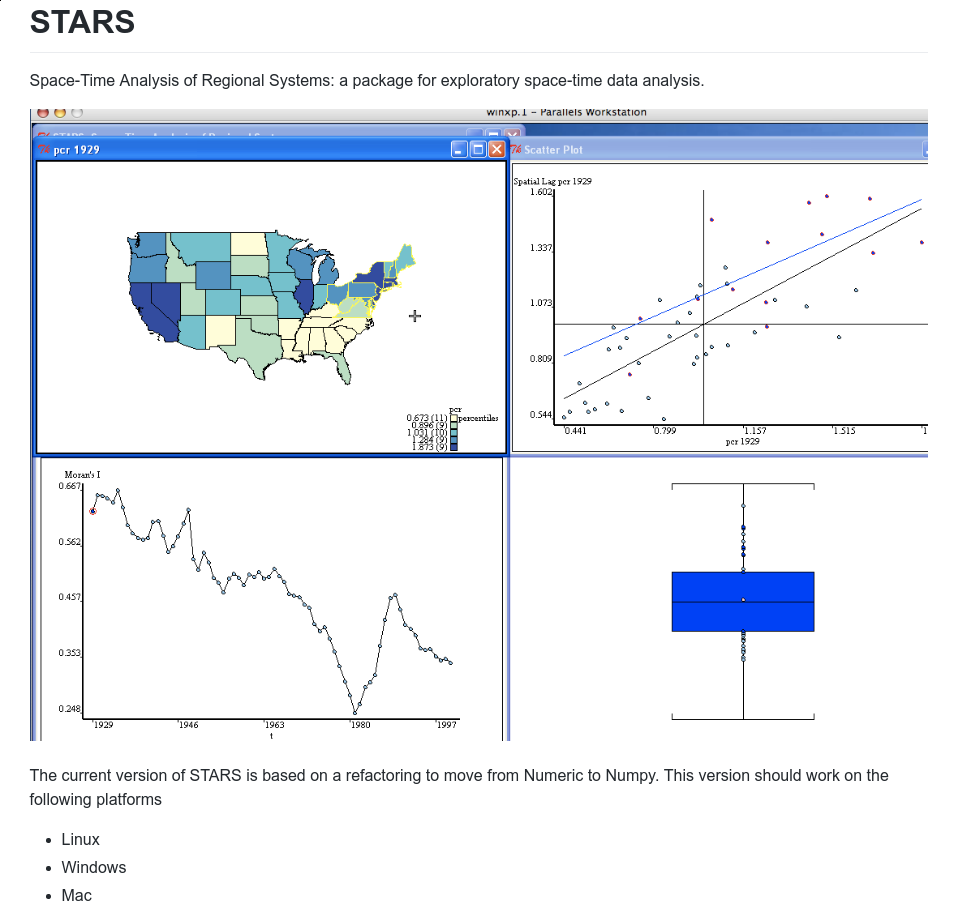
\includegraphics[width=\textwidth,height=0.8\textheight,keepaspectratio]{figures/stars.png}
%   \end{center}
% \end{frame}


\begin{frame}\frametitle{SciPy 2003}
  \begin{center}
    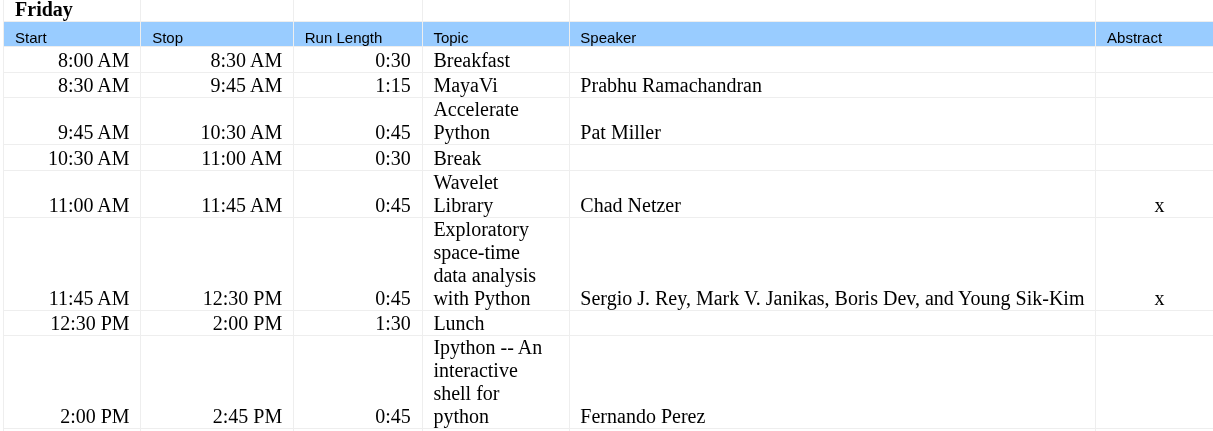
\includegraphics[width=\textwidth,height=0.8\textheight,keepaspectratio]{figures/scipy2003.png}
  \end{center}
\end{frame}



\begin{frame}{PySAL - Layers}
  
  \centering
  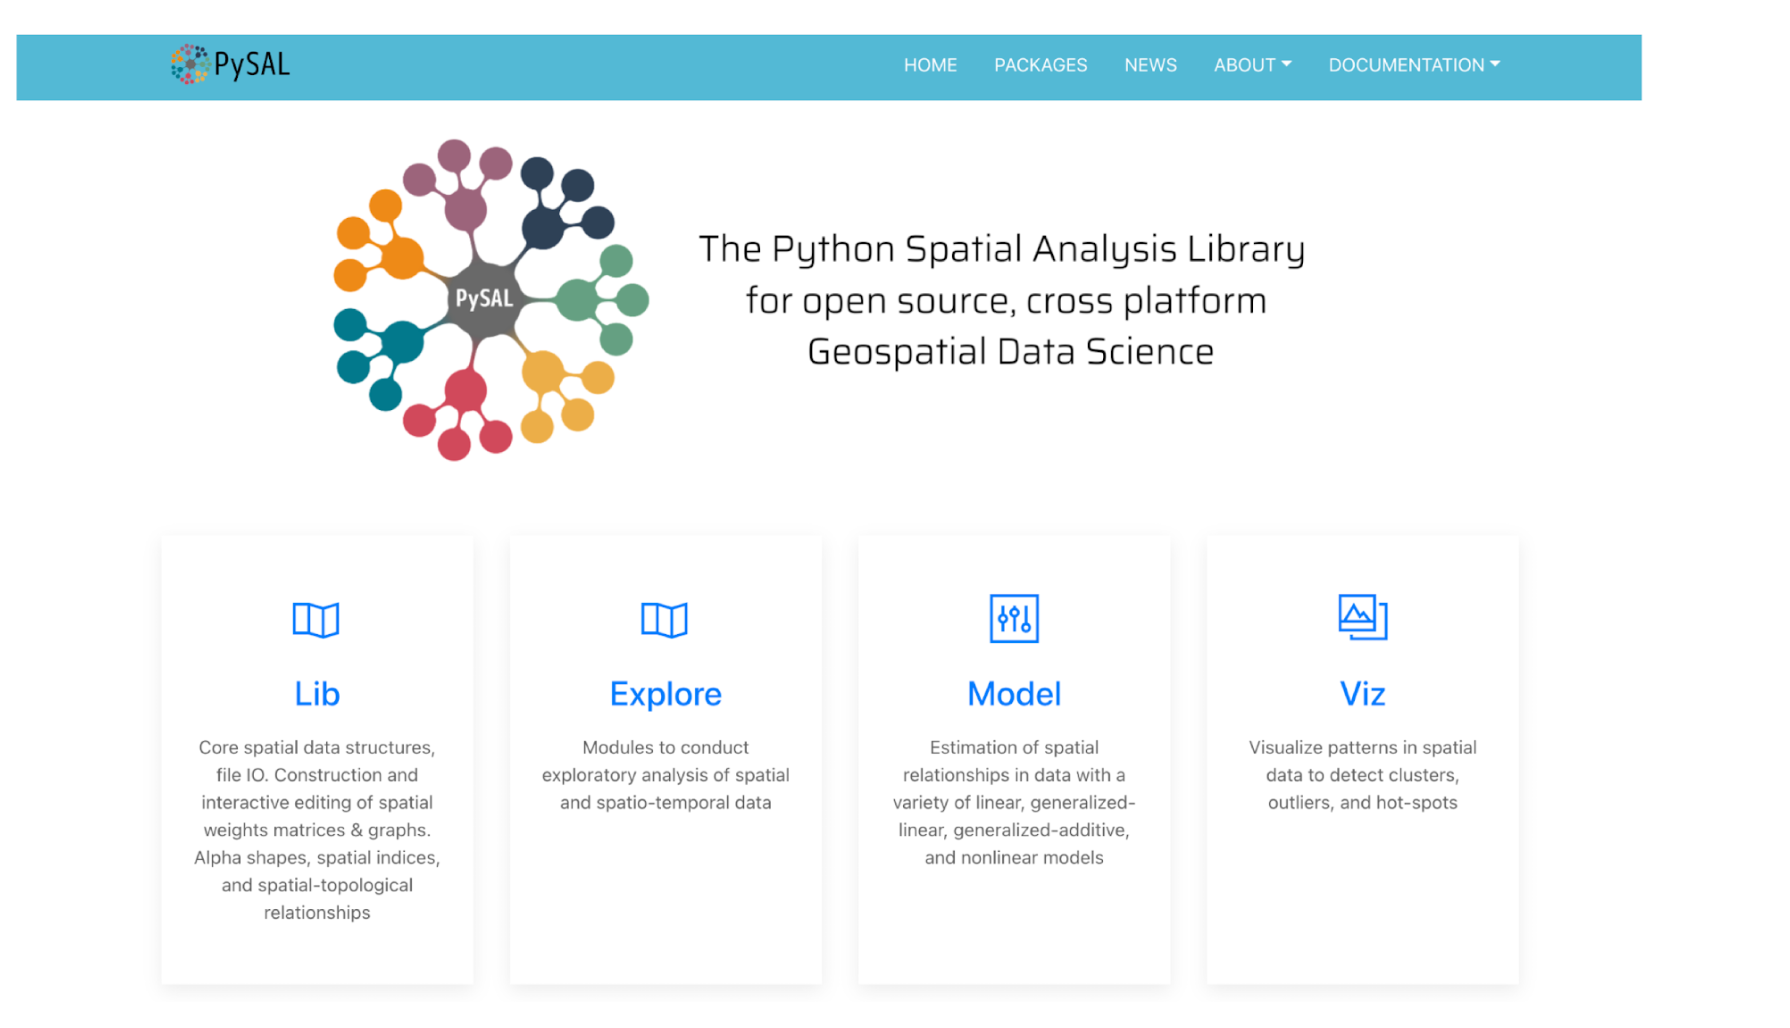
\includegraphics[width=0.8\linewidth]{figures/pysallayers.png} 
  
\end{frame}




\begin{frame}{PySAL libpysal (3 subpackages)}
% Row 1 -------------------------------------------------------------
\modtile{examples}{examples.png}{https://pysal.org/libpysal/}\hfill
\modtile{weights}{weights.png}{https://pysal.org/libpysal/}\hfill
\modtile{graph}{graph.png}{https://pysal.org/libpysal/}\hfill

% Optional footnote-sized caption line
\vspace{0.6em}
\end{frame}


\begin{frame}{PySAL Explore (7 packages)}
% Row 1 -------------------------------------------------------------
\modtile{esda}{esda.png}{https://pysal.org/esda/}\hfill
\modtile{giddy}{giddy.png}{https://pysal.org/giddy/}\hfill
\modtile{inequality}{inequality.png}{https://pysal.org/inequality/}\hfill
\modtile{momepy}{momepy.png}{https://pysal.org/momepy/}

\vspace{0.7em}

% Row 2 -------------------------------------------------------------
\modtile{pointpats}{pointpats.png}{https://pysal.org/pointpats/}\hfill
\modtile{segregation}{segregation.png}{https://pysal.org/segregation/}\hfill
\modtile{spaghetti}{spaghetti.png}{https://pysal.org/spaghetti/}\hfill

% Optional footnote-sized caption line
\vspace{0.6em}
\end{frame}




\begin{frame}{PySAL Model (8 packages)}
% Row 1 -------------------------------------------------------------
\modtile{access}{access.png}{https://pysal.org/access/}\hfill
\modtile{mgwr}{mgwr.png}{https://pysal.org/mgwr/}\hfill
\modtile{spglm}{spglm.png}{https://pysal.org/spglm/}\hfill
\modtile{spint}{spint.png}{https://pysal.org/spint/}

\vspace{0.7em}

% Row 2 -------------------------------------------------------------
\modtile{spopt}{spopt.png}{https://pysal.org/spopt/}\hfill
\modtile{spreg}{spreg.png}{https://pysal.org/spreg/}\hfill
\modtile{spvcm}{spvcm.png}{https://pysal.org/spvcm/}\hfill
\modtile{tobler}{tobler.png}{https://pysal.org/tobler/}

% Optional footnote-sized caption line
\vspace{0.6em}
\end{frame}

\begin{frame}{PySAL Viz (3 packages)}
% Row 1 -------------------------------------------------------------
\modtile{legendgram}{legend.png}{https://pysal.org/legendgram/}\hfill
\modtile{mapclassify}{mapclass.png}{https://pysal.org/mapclassify/}\hfill
\modtile{splot}{splot.png}{https://pysal.org/splot/}\hfill

% Optional footnote-sized caption line
\vspace{0.6em}
\end{frame}


\begin{frame}{Team}
  \centering
  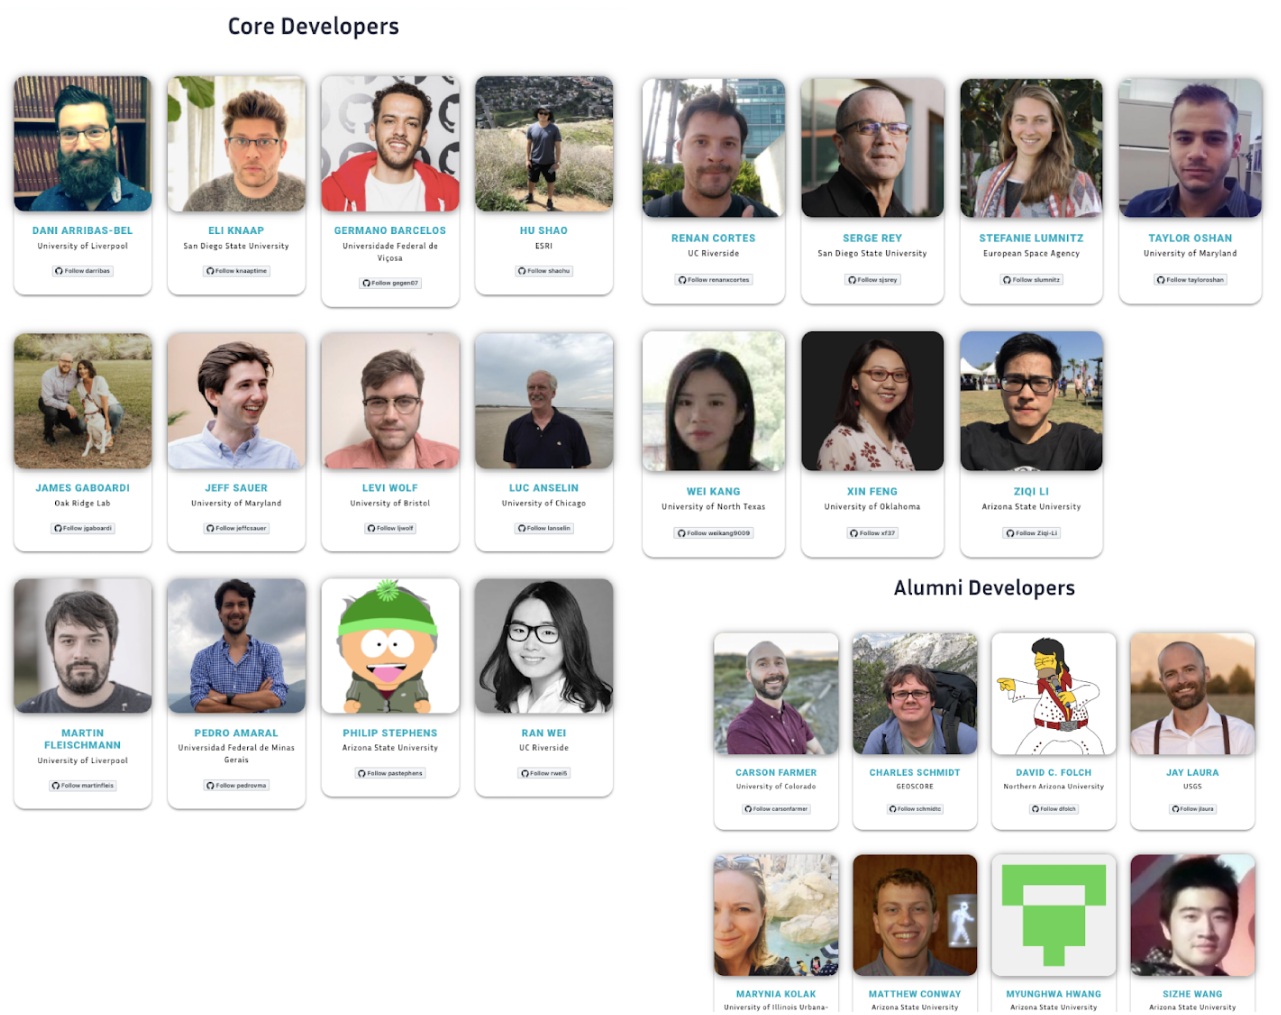
\includegraphics[width=0.7\linewidth]{figures/team.png} 
\end{frame}


\begin{frame}{Thanks  Jupyter and SciPy}

 \begin{block}{PySAL has benefited from being embedded in four interrelated currents}

\begin{itemize}
\item Open Source
\item Open Science
\item Open Education
\item Community
\end{itemize}
\end{block}


\end{frame}

\begin{frame}{Opportunities}
\centering
\vspace{0.5cm}

\begin{columns}[T,onlytextwidth]

% --- Column 1 ---
\begin{column}{0.32\textwidth}
\textbf{Wider Python Scientific Ecosystem}

\vspace{0.4cm}
\begin{itemize}
\item Scientific Python domain stack
\item NumPy SciPy
\item Pandas
\item NetworkX
\item Jupyter ecosystem
\end{itemize}

\vspace{0.3cm}
{\small \textit{Latent synergy:}}\\
Shared numerical infrastructure, graph models, scalable compute patterns
\end{column}

% --- Column 2 ---
\begin{column}{0.32\textwidth}
\textbf{Geo Stack}

\vspace{0.4cm}
\begin{itemize}
\item GeoPandas
\item xarray
\item Pangeo
\item lonboard
\item GeoJupyter
\end{itemize}

\vspace{0.3cm}
{\small \textit{Latent synergy:}}\\
Shared data models, cloud-native geospatial workflows, interactive mapping
\end{column}

% --- Column 3 ---
\begin{column}{0.32\textwidth}
\textbf{Interoperability}

\vspace{0.4cm}
\begin{itemize}
\item R spatial ecosystem (sf, terra)
\item JuliaGeo
\item Cross-language APIs
\item Shared standards
\end{itemize}

\vspace{0.3cm}
{\small \textit{Latent synergy:}}\\
Common data exchange, reproducibility, cross-community collaboration
\end{column}

\end{columns}

\vspace{0.6cm}
\centering
{\large The opportunity is not new tools — it is integration.}

\end{frame}


\begin{frame}{Challenges}
\centering
\vspace{0.4cm}

\begin{columns}[T,onlytextwidth]
  \begin{column}{0.48\textwidth}
    \textbf{Ecosystem-Level Friction}
    \vspace{0.3cm}
    \begin{itemize}
      \item \textbf{Discoverability:} hard to find the “right” tool, example, or workflow
      \item \textbf{Duplication:} parallel implementations, fragmented efforts, incompatible APIs
      \item \textbf{Overload:} too many choices, rapid churn, unclear best practices
      \item \textbf{Integration debt:} glue code, brittle pipelines, version incompatibilities
    \end{itemize}
  \end{column}

  \begin{column}{0.48\textwidth}
    \textbf{Community \& Sustainability Risks}
    \vspace{0.3cm}
    \begin{itemize}
      \item \textbf{Burnout:} small maintainer cores carrying outsized responsibility
      \item \textbf{Invisible labor:} triage, reviews, docs, community support
      \item \textbf{Governance gaps:} unclear decision rights, priorities, succession
      \item \textbf{Funding fragility:} grant cycles, short-term incentives, misaligned support
    \end{itemize}
  \end{column}
\end{columns}

\vspace{0.6cm}
{\large The challenge is not innovation — it is \textbf{sustainable coordination}.}

\end{frame}

\begin{frame}{POSE Project}
  
  \centering
  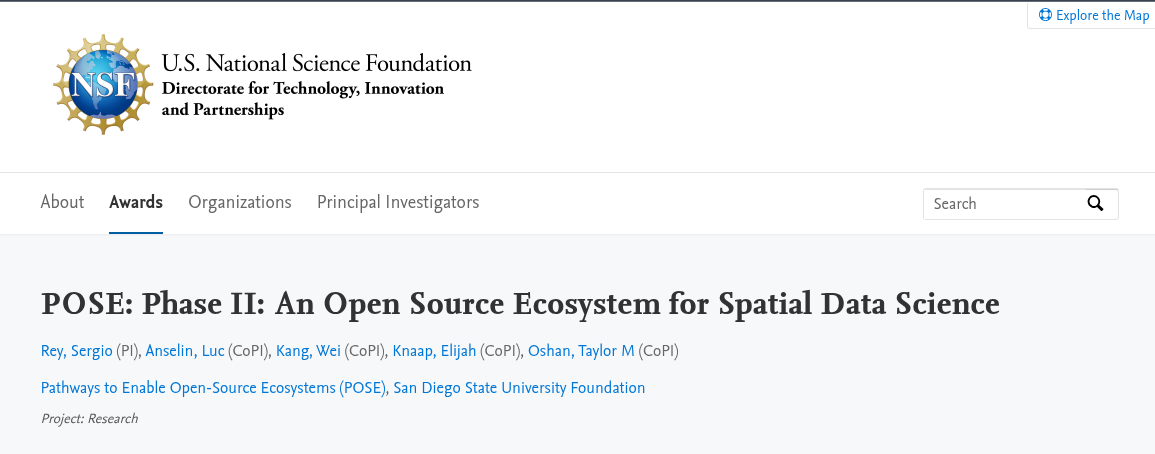
\includegraphics[width=0.7\linewidth]{figures/pose.png} 
\end{frame}


\begin{frame}{Framework}
  
  \centering
  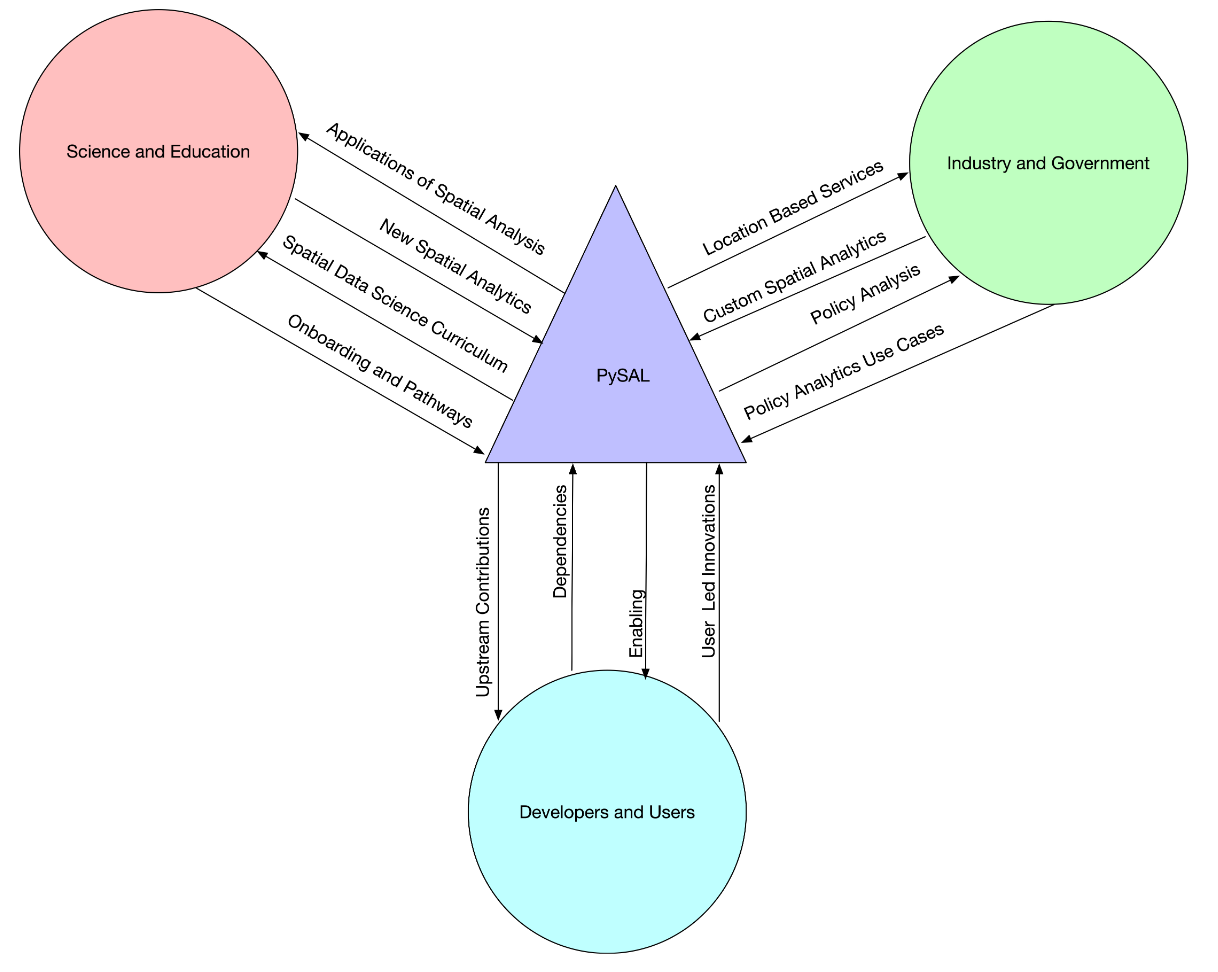
\includegraphics[width=0.7\linewidth]{figures/posefw.png} 
\end{frame}


% \begin{frame}{PySAL: A Modular Toolkit}
    
%     \textbf{PySAL} integrates seamlessly with the PyData stack.
    
%     \vspace{1em}
%     \begin{columns}[T, onlytextwidth]
        
%         \begin{column}{0.32\textwidth}
%             \centering
%             \textbf{1. Data \& Prep}
%             \begin{itemize}
%                 \item \textbf{GeoPandas:} Geospatial dataframes.
%                 \item \textbf{\texttt{libpysal}} (Core): Spatial analysis primitives.
%             \end{itemize}
%             \pause
%             \small
%             \textit{Crucial First Step: Defining \textbf{neighbors} using \texttt{libpysal.graph}.}
%         \end{column}
        
%         \begin{column}{0.32\textwidth}
%             \centering
%             \textbf{2. Exploration (ESDA)}
%             \begin{itemize}
%                 \item \textbf{\texttt{esda}} (Exploratory Spatial Data Analysis).
%                 \item \textbf{Key Tool:} Local Moran's I (identifies hot/cold spots).
%             \end{itemize}
%             \pause
%             \small
%             \textit{Goal: Find patterns.}
%         \end{column}
        
%         \begin{column}{0.32\textwidth}
%             \centering
%             \textbf{3. Modeling (Regression)}
%             \begin{itemize}
%                 \item \textbf{\texttt{spreg}} (Spatial Regression).
%                 \item \textbf{Key Tool:} Spatial Lag / Error Models.
%             \end{itemize}
%             \pause
%             \small
%             \textit{Goal: Build better models.}
%         \end{column}
%     \end{columns}

% \end{frame}

% ----------------------------------------------------
% Section IV: Live Demo 1 (7 min)
% ----------------------------------------------------
\section{What and When?} %11-15

\note{10 minutes
  overview of summit organization
  stress this is flexible
  schedule
}
% \begin{frame}[fragile]{Finding Hot Spots with Local Moran's I}
%   \begin{columns}[t]
%         \begin{column}{0.45\textwidth}
%             \textbf{Goal:} Identify where high values cluster with other high values (Hot Spots), and where low values cluster with other low values (Cold Spots).
%             \vspace{0.5em}
%             \begin{enumerate}
%                 \item \textbf{Load Data:} Crime rates (or housing prices) for US counties.
%                 \item \textbf{Define Neighbors:} Create a Queen contiguity graph.
%                 \item \textbf{Calculate Statistic:} Run \texttt{Moran\_Local} on the variable.
%                 \item \textbf{Map Results:} Plot clusters using GeoPandas.
%             \end{enumerate}
%         \end{column}
        
%         \begin{column}{0.55\textwidth}
%             \textbf{Code}
%             \footnotesize
%             \begin{verbatim}
% import matplotlib.pyplot as plt
% import geopandas as gpd
% from libpysal.graph import Graph
% from esda.moran import Moran_Local
% from splot.esda import plot_local_autocorrelation

% gdf = gpd.read_file(`natregimes.shp')
% queen = Graph.build_contiguity(gdf, rook=False)
% queen = queen.transform(`r')
% li = Moran_Local(gdf.MFI89, queen)
% plot_local_autocorrelation(li, gdf, `MFI89')

%             \end{verbatim}
%         \end{column}
%     \end{columns}
% \end{frame}

% \begin{frame}{Spatial Graph}
%   \centering
%   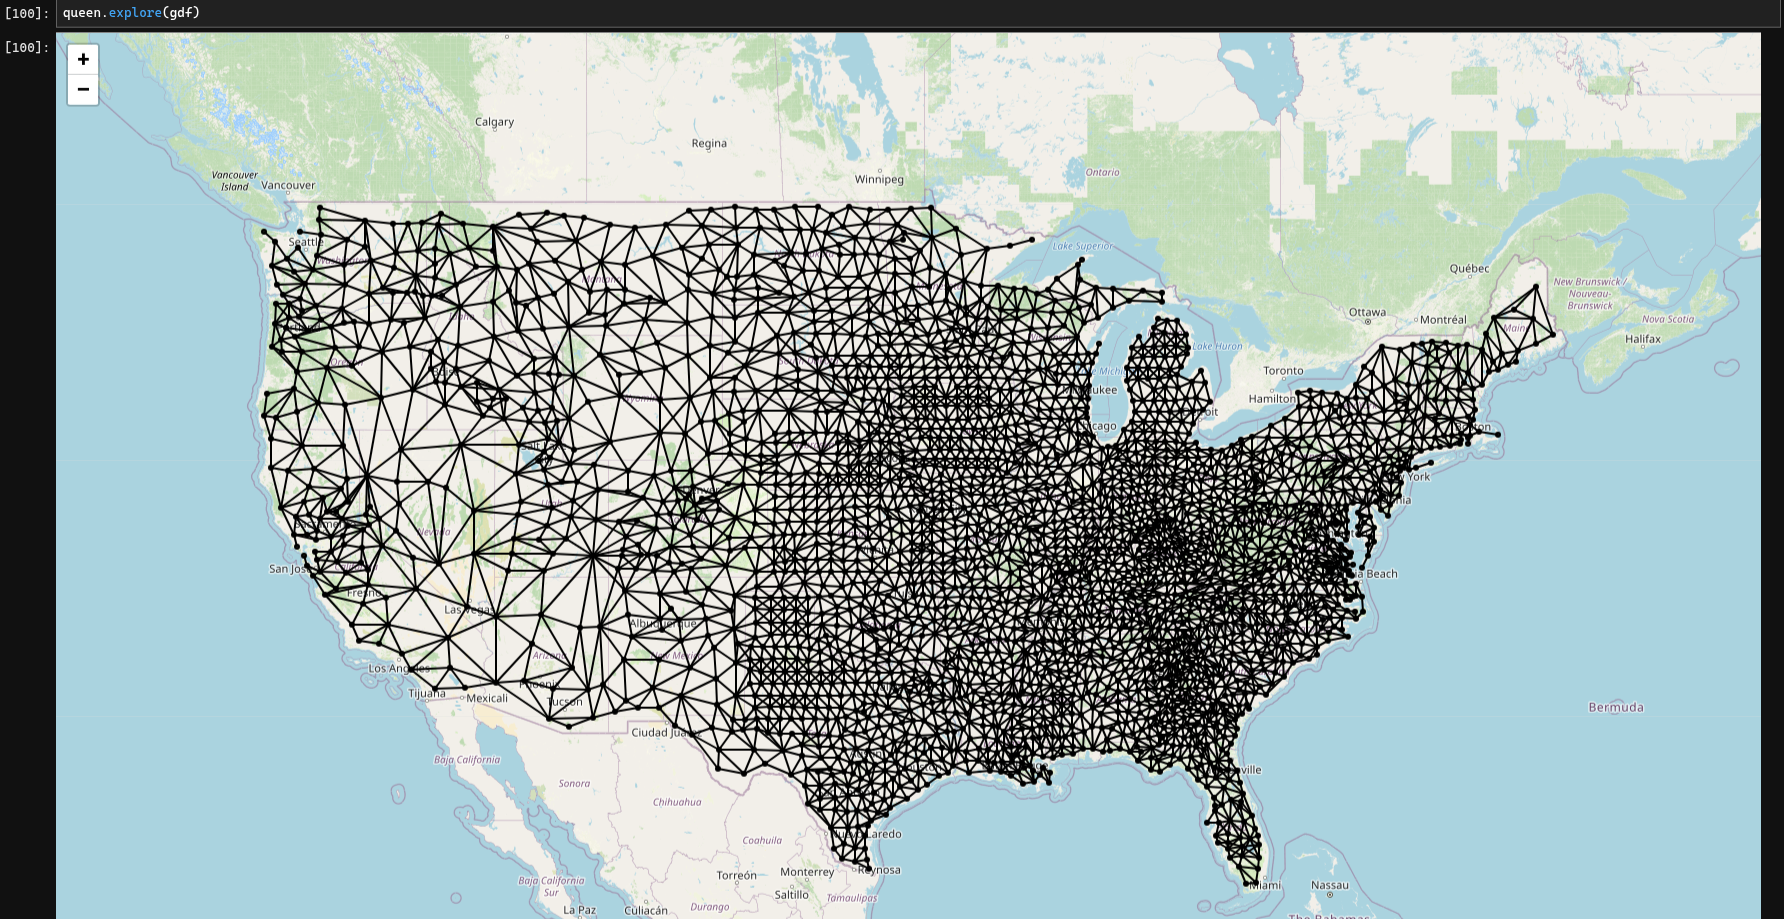
\includegraphics[width=0.8\linewidth]{figures/queen.png} 
% \end{frame}

% \begin{frame}{Hot Spot Analysis}
%   \centering
%   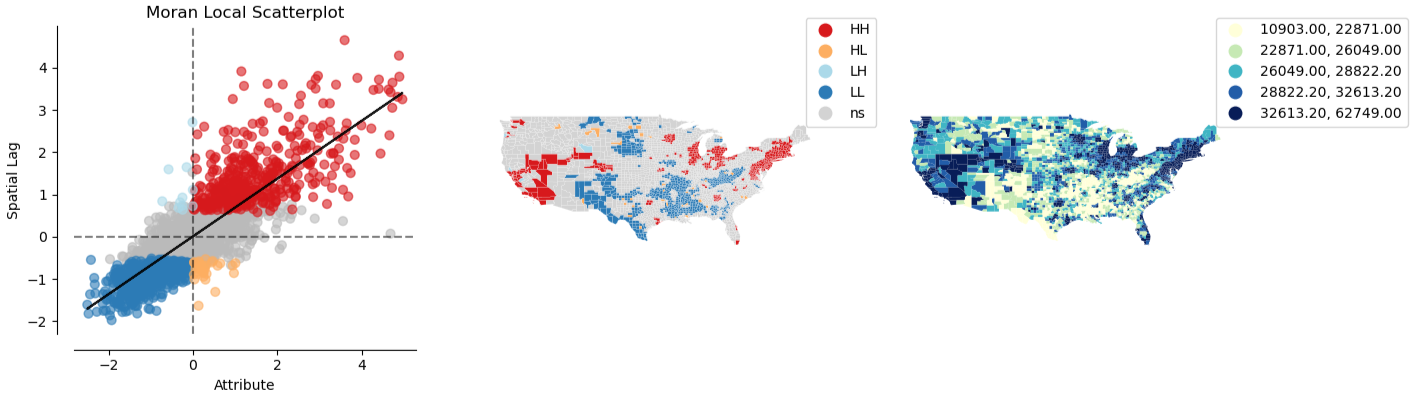
\includegraphics[width=0.9\linewidth]{figures/splot1.png} 
% \end{frame}


% % ----------------------------------------------------
% % Section V: Live Demo 2 (8 min)
% % ----------------------------------------------------
% %\section{Live Demo 2: Spatial Regression} %15-20

% %\begin{frame}[fragile]{Building a Model that 'Listens to Neighbors'}
% %    \begin{columns}
% %        \begin{column}{0.48\textwidth}
% %            \textbf{The Problem:} Our dependent variable ($Y$) might be influenced by the $Y$-values of its neighbors.
% %
% %            \vspace{0.5em}
% %            \textbf{The Solution: Spatial Lag Model}
% %            \vspace{0.5em}
% %            
% %            This model adds a term ($WY$), the weighted average of the neighbor's dependent variable, to the equation.
% %            
% %            \[
% %            Y = \rho WY + X\beta + \epsilon
% %            \]
% %            \uncover<3->{
% %            \textbf{The Takeaway:}
% %            \begin{itemize}
% %                \item Compare OLS to Spatial Lag results.
% %                \item Show how the $\rho$ coefficient reveals spatial dependence.
% %                \item The Spatial Lag model yields better diagnostics.
% %            \end{itemize}}
% %        \end{column}
% %        
% %        \begin{column}{0.52\textwidth}
% %            \textbf{Code Example: Comparing OLS and Spatial Lag}
% %            \begin{verbatim}
% %#| code-fold: true
% %from spreg import OLS, ML_Lag
% %import numpy as np
% %
% %# Simulate data setup
% %# y = data['crime']
% %# X = data[['income', 'density']].values
% %# w = Queen.from_dataframe(data)
% %
% %# 1. Standard OLS
% %# ols_model = OLS(y, X, name_y='crime', name_x=['income', 'density'])
% %# print("--- OLS Model Summary ---")
% %# print(ols_model.summary) 
% %
% %# 2. Spatial Lag Model
% %# lag_model = ML_Lag(y, X, w, name_y='crime', name_x=['income', 'density'])
% %# print("\n--- Spatial Lag Model Summary ---")
% %# print(lag_model.summary) 
% %
% %print("Comparison of R-squared and rho...")
% %            \end{verbatim}
% %        \end{column}
% %    \end{columns}
% %\end{frame}
% %
% % ----------------------------------------------------
% % Section VI: Conclusion (3 min)
% % ----------------------------------------------------


% %\begin{frame}{Bonus Takeaway}
% %\begin{quotation}
% %A couple of months in the laboratory can frequently save a couple of hours in the library.
% %            \textbf{— Frank Westheimer}
% %            \end{quotation}
% %
% %            \pause
% %\begin{quotation}
% %A couple of prompts to the bot and ensuing travels down rabbit holes/dead ends can frequently save you from learning something for yourself.
% %            \textbf{— Me}
% %            \end{quotation}
% %
% %
%\end{frame}

% \begin{frame}{Resources}
%   \centering
%   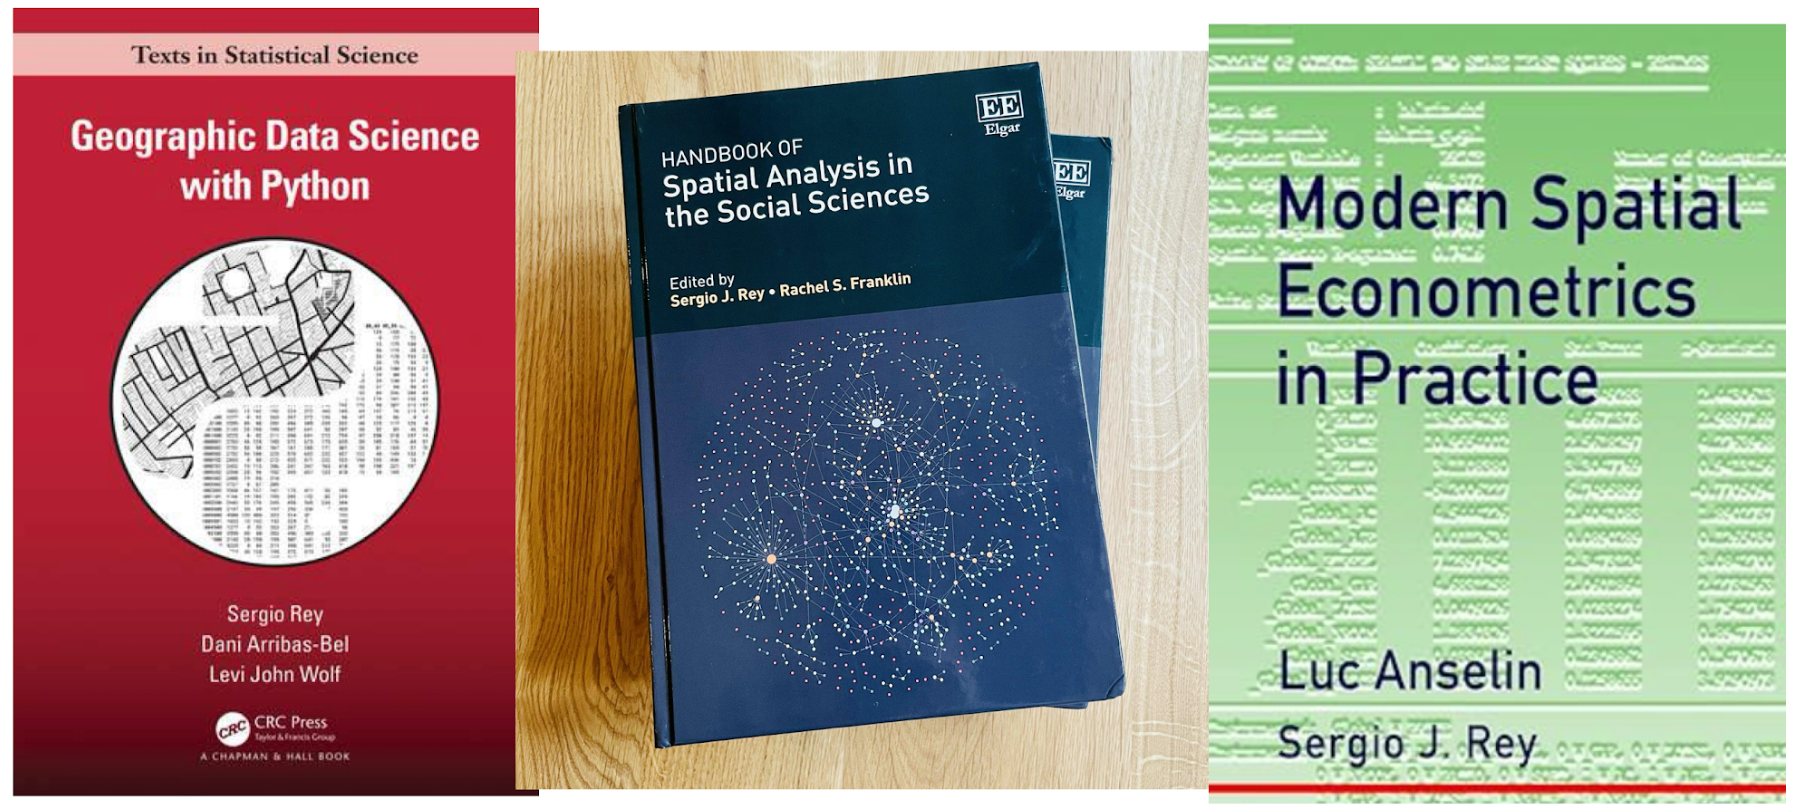
\includegraphics[width=0.7\linewidth]{figures/books.png} 
% \end{frame}

% \begin{frame}{Thank You!}
% \centering
% \begin{tabular}{@{}cll@{}}
%   \faGlobe &PySAL& \href{https://pysal.org}{pysal.org} \\
%   \faGlobe & COGS&\href{https://cogs.sdsu.edu}{cogs.sdsu.edu} \\
%   \faGlobe &Book& \href{https://geographicdata.science/}{geographicdata.science} \\
%   \faGlobe &Me& \href{https://sergerey.org}{sergerey.org} \\
% \end{tabular}
% \end{frame}



% Slide: Sunday header
\begin{frame}{Sunday — March 15}
  \large
  \begin{itemize}
    \item Summit Introduction \hfill 09:00 -- 10:30\\
      \quad General welcome, discuss goals, logistics, intros.  
    \item Break \hfill 10:30-11:30\\
    \item Ecosystem Mapping I \hfill 11:00 -- 12:00\\
    \item Lunch on-site \hfill 12:00 -- 13:00
    \item Afternoon Parallel Sessions \hfill 13:00 -- 14:30\\
      Ecosystem Mapping II — three parallel sessions:
      \begin{itemize}
        \item Science
        \item Education
        \item Industry and Government
      \end{itemize}
    \item Coffee \hfill 14:30 -- 15:00
    \item Ecosystem Mapping III \hfill 15:00 -- 16:30\\
      \quad Synthesize and Prioritize — identify challenges and major points from previous sessions.
    \item Summit Dinner at Eureka \hfill 17:30 -- 19:30
  \end{itemize}

  \note{
    For the Introduction, emphasize summit goals and desired outcomes (3--5 prioritized interventions,
    12--24 month roadmap, working groups). For Ecosystem Mapping sessions, ensure facilitators know
    the deliverable format: each group should identify key projects, gaps, and 2--3 near-term actions.
    Remind participants about the dinner logistics and transport if needed.
  }
\end{frame}

% Slide: Sunday — Ecosystem Mapping I detail
\begin{frame}{Ecosystem Mapping I — (10:30--12:00)}
  \begin{itemize}
    \item Purpose: inventory projects, tools, and institutions across the ecosystem.
    \item Focus areas:
      \begin{itemize}
        \item Where PySAL is applied in science.
        \item Teaching uses and pedagogical materials.
        \item Government applications and operational use cases.
      \end{itemize}
    \item Expected output: short list of current initiatives and major gaps.
  \end{itemize}

  \note{
    Encourage participants to call out existing efforts, dependencies, and "bridge" projects.
    Capture representative examples and contacts for follow-up.
  }
\end{frame}

% Slide: Sunday — Afternoon Parallel Sessions detail
\begin{frame}{Ecosystem Mapping II — Parallel Sessions (13:00--14:30)}
  \begin{itemize}
    \item Three parallel tracks:
      \begin{enumerate}
        \item Science — methods, reproducibility, cross-disciplinary problems.
        \item Education — curriculum, modular materials, instructor support.
        \item Industry \& Government — adoption pathways, procurement friction, real-world pilots.
      \end{enumerate}
    \item Each session: facilitator, note-taker, 3–4 discussion prompts, and a brief report-out.
  \end{itemize}

  \note{
    Remind facilitators to timebox conversation and capture 2–3 priority actions or needs to bring
    to the Synthesis session.
  }
\end{frame}

% Slide: Sunday — Ecosystem Mapping III detail
\begin{frame}{Ecosystem Mapping III — Synthesize \& Prioritize (15:00--16:30)}
  \begin{itemize}
    \item Synthesize findings across the three tracks.
    \item Prioritize major challenges and leverage points.
    \item Form preliminary working group ideas for Day 2.
  \end{itemize}

  \note{
    The aim is to converge on a short list of cross-cutting priorities that will seed the Day 2
    working groups (governance, interoperability, education pipelines, adoption pathways, etc.).
  }
\end{frame}

% Slide: Sunday evening
\begin{frame}{Sunday Evening}
  \begin{itemize}
    \item Summit Dinner — Eureka \hfill 17:30 -- 19:30
    \item Informal conversations and networking
  \end{itemize}

  \note{
    Ensure attendees know the meeting point and transportation if needed. Use this time to
    recruit working group volunteers and encourage informal cross-domain discussions.
  }
\end{frame}

% Slide: Monday header
\begin{frame}{Monday — March 16}
  \large
  \begin{itemize}
    \item Breakfast on-site \hfill 08:00 -- 09:00
    \item Introduction / Reground \hfill 09:00 -- 09:30\\
      \quad Reflect on Day 1 and prepare for Day 2 topics.
    \item Parallel Working Groups \hfill 09:30 -- 11:30
    \item Community PySAL Book working group \\
      \quad Define purpose, scope, and process.
    \item Shared Teaching Materials working group \\
      \quad Design infrastructure to create, share, and coordinate materials.
    \item Lunch on-site \hfill 11:30 -- 13:00
    \item Midday Cross-Group Collaboration \hfill 13:00 -- 14:30\\
      \quad Ecosystem, Book, and Teaching groups mix to discuss plans and feasibility.
    \item Coffee \hfill 14:30 -- 15:00
    \item Final Group Collaboration \hfill 15:00 -- 16:30\\
      \quad Finalize ecosystem interventions, book initiatives, and teaching materials.
    \item Next Steps + Closing \hfill 16:30 -- 17:00\\
      \quad Summarize commitments and timelines.
  \end{itemize}

  \note{
    For Monday working groups, be explicit about scope and expected outputs: charters,
    short-term milestones, and volunteers to lead initial meetings. The book group should
    draft a one-page scope and editorial process during the session.
  }
\end{frame}

% Slide: Monday — Working Groups detail
\begin{frame}{Parallel Working Groups (09:30--11:30)}
  \begin{itemize}
    \item Governance and Sustainability\\
      \quad Focus: governance model, funding diversification, maintainers' pipeline.
    \item Interoperability and Standards Coordination\\
      \quad Focus: data models, interchange formats (GeoDataFrame, xarray), API conventions.
    \item Education to Contribution Pipelines\\
      \quad Focus: curriculum → contributor pathways, modular teaching assets.
    \item Industry and Government Adoption Pathways\\
      \quad Focus: procurement, enterprise integration, pilot projects.
  \end{itemize}

  \note{
    Each group should produce a 1-page output: problem statement, three priority actions, and
    named volunteers for the next 90 days.
  }
\end{frame}

% Slide: Monday — Community Book \& Teaching groups
\begin{frame}{Community PySAL Book \& Shared Teaching Materials}
  \begin{itemize}
    \item Community PySAL Book Working Group (09:30--11:30)\\
      \quad Define purpose, scope, chapter outlines, authorship model, and timeline.
    \item Shared Teaching Materials Working Group (09:30--11:30)\\
      \quad Design infrastructure to create, host, and coordinate reusable notebooks and assignments.
  \end{itemize}

  \note{
    For the book group: decide licensing, editorial board, and minimal chapter template.
    For teaching materials: consider a central repo, CI for tests, and templates for assessments.
  }
\end{frame}

% Slide: Monday — Midday Cross-Group Collaboration
\begin{frame}{Midday Cross-Group Collaboration (13:00--14:30)}
  \begin{itemize}
    \item Mix members from Ecosystem groups, Book group, and Teaching group.
    \item Discuss feasibility, resource needs, and coordination mechanisms.
    \item Identify immediate pilot projects and initial owners.
  \end{itemize}

  \note{
    This session is to ensure alignment across outputs and to identify overlapping responsibilities,
    avoiding duplication and ensuring leverage.
  }
\end{frame}

% Slide: Monday — Final Collaboration + Next Steps
\begin{frame}{Final Collaboration (15:00--16:30) \& Closing (16:30--17:00)}
  \begin{itemize}
    \item Finalize interventions and working group charters.
    \item Clarify outputs, timelines, and who is responsible.
    \item Commit to short-term milestones (first 90 days).
    \item Closing: summarize commitments and next steps.
  \end{itemize}

  \note{
    Capture assignments in a shared doc; schedule the first follow-up working group meetings
    before attendees depart. Announce where minutes and materials will be posted.
  }
\end{frame}

\section{Who and How?}
\note{40 minutes introductions
10 minutes logistics}
\begin{frame}
  \frametitle{Participant Introductions}
  
\begin{itemize}
\item \textbf{Name + Institution}
\item \textbf{Where You Sit in the Ecosystem}
\item \textbf{What Gap You See}
\item \textbf{What You’re Willing to Help Build}
 
\end{itemize}
\note{Keep to 1 minutes max

  Segue via introduction of students and into logistics 
}

\note{Thank you — that was efficient and very helpful.

We now have a clearer sense of who is in the room and what each of you is bringing.

Before we begin the substantive ecosystem work, let’s take five minutes to cover logistical details so we can focus fully once we reconvene.

After that, we’ll take a short break — and when we return, we’ll move directly into Ecosystem Mapping I.}
\end{frame}
% Logistics slide
\begin{frame}{Logistics}
  \begin{itemize}
    \item Meals: breakfast and lunch on-site; coffee breaks as scheduled.
    \item Wifi
    \item Accessibility \& dietary needs
    \item Discord
    \item Reimbursement Process
  \end{itemize}

  \note{
    Provide the registration desk phone number and local contact for same-day issues.
    Remind participants about submitting travel/arrival info if needed.
  }
\end{frame}

% Closing / Contacts
% \begin{frame}{Closing & Contacts}
%   \begin{itemize}
%     \item Organizing Committee:
%       \begin{itemize}
%         \item Serge Rey
%         \item Eli Knaap
%         \item Wei Kang
%         \item Jarrod Millman
%         \item Maryam Hosseini
%       \end{itemize}
%   \end{itemize}

%   \note{
%     Thank participants for their engagement; remind them to sign up for working groups and
%     to check the program page for slides and materials after the summit.
%   }
% \end{frame}




\end{document}
